% AUTO-GENERATED by writeup/make_rehaul_ladder.py --everybar -- do not edit; re-run the script.
% Figure fig:rh_ladder_everybar: the feature-count ladder refitted at every bar, results/ablations_2014start_w3000/scores_fomcfix
% (results/ablations_2014start_w3000/RULE.txt ADDENDUM K). Label: every-bar refit, requested by the author after the monthly-vs-every-bar comparison; not pre-registered.
\begin{figure}[tbp]
  \centering
  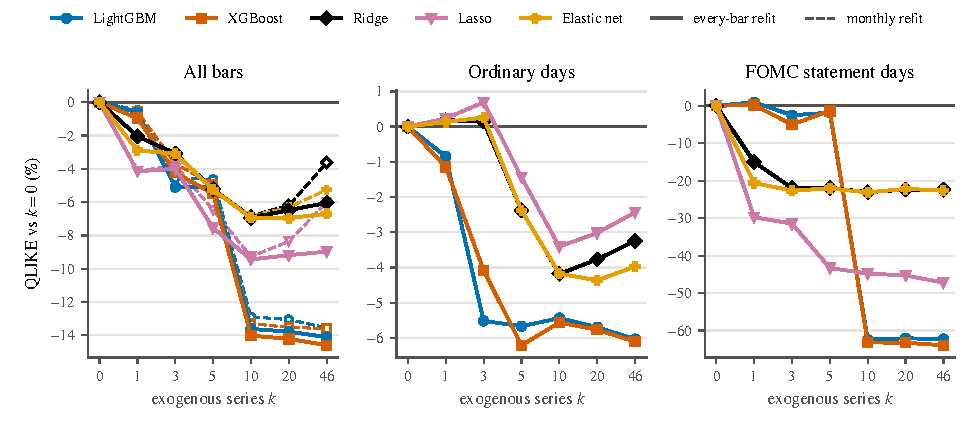
\includegraphics[width=\linewidth]{figures/rehaul_ladder_everybar.pdf}
  \caption{How many exogenous series carry the gain when every rung is refitted at every bar. Each model is refitted
    at every bar on its top $k$ exogenous series only, ranked once by the model's own importance measure on a fit
    explained on \rhldEBRankYear{} data, before the evaluation span; $k = 0$ (the HAR benchmark set) and
    $k = \rhldEBNSeries$ (the full set) are the walks of Table~\ref{tab:rh_oos}. Vertical axis: the QLIKE of the
    rung relative to the same model's $k = 0$ rung, in percent (negative: more accurate), on the \rhldEBNBars{} bars
    of Table~\ref{tab:rh_oos} (left), on the \rhldEBNDaysOrd{} ordinary days (middle) and on the
    \rhldEBNDaysEv{} FOMC statement days (right). Solid: refitted at every bar, window $W = \rhldEBWindowDays$
    trading days, hyperparameters frozen. Dashed (left panel): the same models refitted monthly, the ladder of
    Figure~\ref{fig:rh_ladder}, each against its own $k = 0$ rung. LightGBM, XGBoost and the linear models; no
    random forest. FOMC-patched design. Every-bar refit, requested by the author after the monthly-vs-every-bar
    comparison; not pre-registered.}
  \label{fig:rh_ladder_everybar}
\end{figure}
